\documentclass[landscape]{article}
\usepackage{listings}
\lstset{frameround=fttt,language=Caml,numbers=left,breaklines=true}
\usepackage{latexsym,amsmath,amssymb,stmaryrd}
\usepackage{xspace}
\usepackage{enumerate}
\usepackage{pgf}
\usepackage{mathpartir}
\usepackage{color}
\usepackage{soul}
\usepackage{subscript}
\newcommand{\code}[1]{\text{\lstinline!#1!}}
\usepackage{tikz}
\usetikzlibrary{automata,positioning}
\begin{document}

\section{Bump app}

The bump app allows the email box to be checked.  It is characterized
by the following state transition diagram:

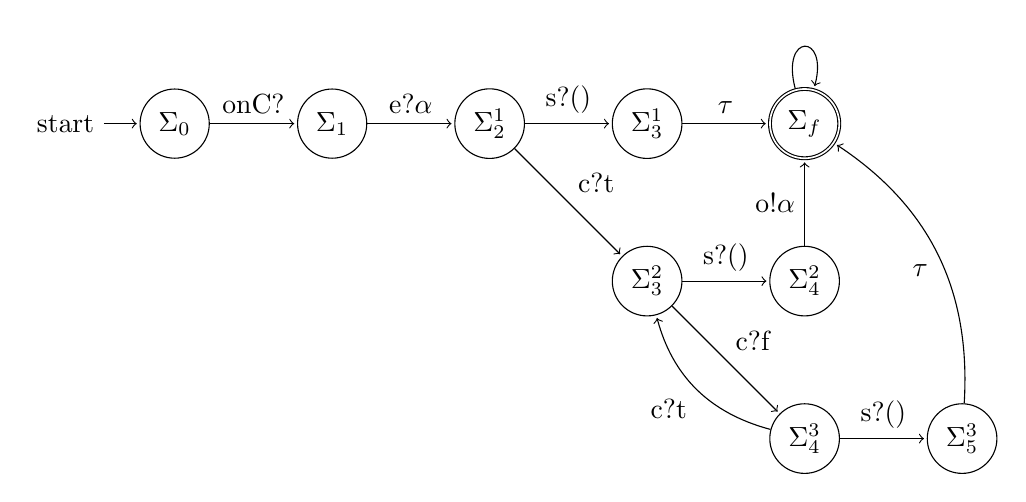
\begin{tikzpicture}[shorten >=1pt,node distance=2cm,on grid,auto] 
   \node[state,initial] (q_0)   {$\Sigma_0$};
   \node[state] (q_1) [right=of q_0] {$\Sigma_1$};
   \node[state] (q_2) [right=of q_1] {$\Sigma_2^1$};
   \node[state] (q_31) [right=of q_2] {$\Sigma_3^1$};
   \node[state] (q_32) [below=of q_31] {$\Sigma_3^2$};
   \node[state] (q_42) [right=of q_32] {$\Sigma_4^2$};
%   \node[state] (q_33) [below=of q_32] {$e_s = \alpha$};
   \node[state] (q_43) [below=of q_42] {$\Sigma_4^3$};
   \node[state] (q_53) [right=of q_43] {$\Sigma_5^3$};
   \node[state,accepting](final) [right=of q_31] {$\Sigma_f$};
    \path[->] 
    (q_0) edge  node {\code{onC?}} (q_1)
    (q_1) edge  node {\code{e?}$\alpha$} (q_2)
    (q_2) edge  node {s?()} (q_31)
          edge  node {c?t} (q_32)
    (q_31) edge node {$\tau$} (final)
    (q_42) edge node {o!$\alpha$} (final)
    (q_32) edge node {s?()} (q_42)
           edge node {c?f} (q_43)
    (q_43) edge node {s?()} (q_53)
           edge [bend left] node {c?t} (q_32)
    (q_53) edge [bend right] node {$\tau$} (final)
    (final) edge [loop above] node {} ();
\end{tikzpicture}

Note that the diagram is schematic in $\alpha$, meaning that any
variable could be substituted.  (As a trivial example, we could
finitize it with a single bit zero or one.)

We now want to argue that the program satisfies noninterference.  We
therefore need to show that for every low input equivalent trace, we
see a low equivalent output.  Note that in this example, we only have
one output (right before the final state) as a simplification.  We now
need to argue that the state space of the diagram above is somehow in
``correspondence'' with the semantics of the program.

To do this, we consider a traversal through the program.  We assume
that the semantics is deterministic and steps from state $\Sigma_0$ to
$\Sigma_2^1$: by first calling the \code{onC} handler, then reading
the value $\alpha$ from the \code{e} channel.

This is the point where one source of nondeterminism happens.  At this
point, the program enters an event loop that responds to two channels
until the program exits: the send button (we call \code{s}), or the
checkbox channel (which we assume has a toggle semantics, meaning it
goes from true to false to true only).  Branching off from state
$\Sigma_2^1$, the program input will have the grammar $G$:

\begin{displaymath}
\begin{array}{ccc}
  I & ::= & Ctrue , s?() \\
  CTrue & ::= & c?t , CFalse \mid \epsilon \\
  CFalse & ::= & c?f , CTrue \mid \epsilon \\
\end{array}
\end{displaymath}

And the output of the final send will depend on the last value on the
\code{c} channel.

First note that in this example, the click handler is ``pure:'' the
state of the program is not affected by the handlers running.  We can
verify this by simply looking at the example code:

\lstset{frameround=fttt,language=Java,numbers=left,breaklines=true}
\begin{lstlisting}
  public void onClick(View v) {
    if (emailBox.isChecked()) {
      InfoSender.sendInt(email);
    }
  }
\end{lstlisting}

Note also that the checkbox handler changes the program state to
update the \code{emailBox.isChecked} variable to be what the value
that was clicked.

Now consider any input sentence $s \in G$:

\begin{itemize}
\item $s?()$, doesn't print anything in the program, and jumps to the
  final state.
\item $c?f, s?()$, doesn't print anything in the program, jumps to the
  final state.
\item $c?f, c?t, s?()$, prints the value $email$.
\item $c?f, ..., c?f, s?()$, doesn't print anything in the program,
  jumps to the final state.  Note that we can see this via the fact
  that the program state toggles from the member variable
  \code{emailBox.isChecked} jumping from false to true with each
  toggle on the channel.
\item $c?f, ..., c?t, s?()$, prints the value $email$.
\end{itemize}

Now, we'd like to use this insight to prove that the program
statisfies noninterference.  This requires $=_{L,in} \Rightarrow =_L$.
Consider any input sequence.  Now, consider the input sequences via
the grammar again, we need to argue that low equivalent input
sequences will lead to low observable output:

\begin{itemize}
\item $s?()$, the low input to the program is simply the event $s?()$.
  There is no low ouput, so $=_L$ trivially holds because $=_{L,in}$
  as assumed to hold.
\item $c?f, s?()$, the low input is exactly the sequence, and for the
  same reason as the last bullet the formula holds.

\item $c?f, c?t, s?()$, the low input is the sequence $e?\alpha, c?f,
  c?t, s?(), o!\alpha$ (this is because the declassification condition
  allowed the email read to go from high to low).  Consider any
  \emph{fixed} value $\alpha$.  It is true that $=_L$ whenever
  $=_{L,in}$, e.g., consider the trivial case where $\alpha$ is simply
  a bit.
\item $c?f, ..., c?f, s?()$, case holds because of the argument that
  the program is in the same state as the second bullet.
\item $c?f, ..., c?t, s?()$, case holds because of the argument that
  the program is in the same state as the third bullet.
\end{itemize}

\section{Bump app (evil 1)}

\begin{lstlisting}
  public void onClick(View v) {
    numPushes += 1;
    if (numPushes >= 2) {
      InfoSender.sendInt(email);
    } 
    if (emailBox.isChecked()) {
      InfoSender.sendInt(email);
    }
  }
\end{lstlisting}

This app has the same behavior, except that the handler for the
\code{onClick} handler is \emph{not} pure.

\end{document}



